
\def\theTopic{Unit 1 Review }
\def\dayNum{9}

\begin{center}
{\bf {\large Unit 1 Review }}
 \\
  {\bf Vocabulary} Define each term:
\end{center}
\begin{itemize}
\item sample
\item population
\item statistic
\item parameter
\item types of variables
\item measures of center
\item measures of spread
\item estimation bias
 \item Null hypothesis 
 \item Alternative hypothesis
\item Strength of evidence 
\begin{key}
{\it
    The probability (proportion of simulations) of results as or
    more extreme as the observed result.}
\end{key}
\item Confidence interval
%%\item margin of error
\end{itemize}



\begin{center}
{\bf  Simulation}
\end{center}
\begin{enumerate}
\item If we repeat the ``Helper -- Hinderer'' study and  10 of
    the 16 infants chose the helper (6 chose hinderer):
    \begin{enumerate}
    \item How would you assess the strength of evidence using the same
      simulation we already performed?
\begin{students}
        \vspace{3.5cm}
\end{students}

\begin{key}
{\it
      Because only the observed result and nothing in the model
      actually changed, there is no reason to re-do the model.  We
      just skip to step 4 and compare the observed result to the
      null distribution. }
\end{key}
\item What strength of evidence against the null hypothesis
      does this new data provide?
\begin{students}
        \vspace{3.5cm}
\end{students}

\begin{key}
{\it
      In my simulation of 1000, there were 238 trials with 10 or
      more picking the helper, which gives a strength of evidence
      of .238 = 23.8\%}
\end{key}
\item If 13 kids chose the helper toy, what is the strength of evidence
  against the null hypothesis? 
\begin{students}
        \vspace{3.5cm}
\end{students}

\begin{key}
{\it
       With a strength of evidence of 9/1000 = .009 = .9\%, I have
      strong evidence against the null model and can conclude that
      infants do in fact use social interactions to pick a toy. }
\end{key}
\item If we redid the study with 8 infants, and 7 chose the
      helper, is this stronger, weaker, or the same amount of evidence
      against the null hypothesis?      
\begin{key}
{\it
      The fraction is the same, but because the sample size is
      smaller, it is less unusual to see 7 of 8 picking helper than
      to see 14 of 16.}
\end{key}
\item Explain how would you rerun the simulation for only 8 infants.
\begin{students}
        \vspace{2cm}
\end{students}
      
\begin{key}
{\it
      Change the number of trials to
      8 instead of 16.   }
\end{key}
\item Perform the simulation for 8 infants and compare the
      strength of evidence provided by 7 choosing the helper.  Was your
      hunch correct?  Explain any differences.      
\begin{students}
        \vspace{3.5cm}
\end{students}

\begin{key}
{\it
      If they said: the same, then a response might be:
      The simulation showed my answer was wrong.  There is less
      spread when the trial size was 16 than when it was 8.  Due to
      the greater spread in trial size 8, there were more trials
      with 7 or more helpers chosen (approximately 40/1000) than
      there were trials with 14 or more helpers chosen out of 16
      (approximately 1/1000). }
\end{key}
\end{enumerate}


\item A German bio-psychologist, Onur G\"{u}nt\"{u}rk\"{u}n, was
  curious whether the human tendency for right-sidedness (e.g.,
  right-handed, right-footed, right-eyed), manifested itself in other
  situations as well. In trying to understand why human brains
  function asymmetrically, with each side controlling different
  abilities, he investigated whether kissing couples were more likely
  to lean their heads to the right than to the left.  He and his
  researchers observed 124 couples (estimated ages 13 to 70 years, not
  holding any other objects like luggage that might influence their
  behavior) in public places such as airports, train stations,
  beaches, and parks in the United States, Germany, and Turkey, of
  which 80 leaned their heads to the right when kissing.
  \begin{enumerate}
    \item  What parameter is of interest?
\begin{students}
    \vspace{1.4cm}    
\end{students}
\begin{key} 
  {\it $p$ = the proportion of all couples who lean right when kissing.}
\end{key}
  \item \label{kiss.phat} What statistic do we obtain from the sample?
    Give proper notation, the statistic's value, and explain it in words.
\begin{students}
    \vspace{2cm}    \\
\end{students}
\begin{key} 
   { $\widehat{p} = \frac{80}{124} = 0.645$ \it is the
    proportion of couples leaning right.}
\end{key}
\item We can set the null hypothesis as we have before, but don't know
  before collecting data whether the alternative should be greater or
  less than one half. We therefore use a ``two-sided'' alternative
  with a $\neq$ sign.
    \begin{enumerate}
    \item State null and alternative hypotheses in symbols and
      words.\\
      $H_0:$ 
\begin{students}
    \vspace{1.5cm}    \\
\end{students}
\begin{key} 
{\it $p = .5$.  Half of all couples lean right when kissing.}
\end{key}
$H_a:$
\begin{students}
    \vspace{1cm}    \\
\end{students}
\begin{key} 
{\it $p \neq .5$.  The true proportion of couples leaning right when
  kissing is not one half.}
\end{key}
    \item How would you mark cards and randomly draw from them to
      obtain one simulated proportion drawn from the distribution when
      $H_0$ is true?
\begin{students}
    \vspace{3cm}    
\end{students}
\begin{key} 
{\it Take an even number of cards (could be 124, but a
    smaller number will also work). Mark half of them right, half
    left. Shuffle and draw one. Record the lean. Return the card
    to the deck, repeat 123 more times and divide the total number of
    right's by 124 to get one sample proportion.}
\end{key}
    \item Use the  \fbox{One Categ} -- \fbox{Test} applet to obtain
      the distribution of 1000 or more sample proportions under $H_0$.
      Sketch the picture you get here.
\begin{students}
    \vspace{5cm}    
\end{students}
\begin{key}
\ \  \\ 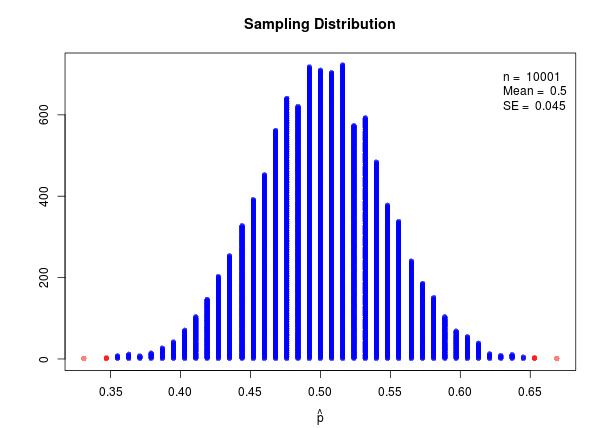
\includegraphics[width=.3\linewidth]{../plots/kissing-null.png}
\end{key}
  \item How unusual is the sample statistic from \ref{kiss.phat}
    relative to the distribution you created?  Explain in words where
    it falls relative to the plotted points.
\begin{students}
    \vspace{3cm}    
\end{students}

\begin{key}
{\it Only 8 of the 10000 points I generated are this extreme.}
\end{key} 
\item  How strong is the evidence against the null hypothesis?  What
  do you think about the idea that only half of couples lean right
  when kissing?
\begin{students}
    \vspace{2cm}    
\end{students}

\begin{key}
  {\it Extremely strong evidence, the p-value is 0.0008 which is less than 1 in
    1000. The null hypothesis of half leaning right is not consistent
    with these data. I conclude that  more than half of kissing
    couples lean to the right.  } 
\end{key}


\end{enumerate}

\item Now estimate the true population proportion.
  \begin{enumerate}
    \item What is our ``point'' estimate of the
      true proportion of couples who lean right?
\begin{students}
    \vspace{.4cm}    
\end{students}

\begin{key}
$\widehat{p} = 0.645$
\end{key}
    \item In order to generate simulated data,
      \begin{enumerate}
        \item How many couples do we generate for one resample?
\begin{students}
    \vspace{.8cm}    
\end{students}

\begin{key} 
$124$
\end{key}
       \item Explain how you would mark 124 cards and use them to
         simulate the lean of one couple, and then another.
\begin{students}
    \vspace{2.5cm}    
\end{students}

\begin{key} 
  {\it Mark 44 ``Left'' and 80 ``Right''.  Shuffle them and draw one at
    random and write down the lean on the selected card.  Replace the
    card, remix, and draw again for the second person.}
\end{key}
       \item Each couple leans right with what probability?
\begin{students}
    \vspace{.5cm}    
\end{students}

\begin{key} 
  {$0.645$}
\end{key}
       \item After resampling 124 individuals, what number would you compute?
\begin{students}
    \vspace{1.2cm}    
\end{students}

\begin{key} 
  {\it  The proportion of the 124 new draws which are right.}
\end{key}
     \end{enumerate}
     \item Use the  web applet to create  1000 or more
       resamples from the original data.
       \begin{enumerate}
         \item Where is this distribution centered?
\begin{students}
    \vspace{.7cm}    
\end{students}

\begin{key} 
  {\it  0.645}
\end{key}
         \item What number describes the spread of the distribution?
\begin{students}
    \vspace{.7cm}    
\end{students}

\begin{key} 
  {\it SE =  0.045}
\end{key}
         \end{enumerate}
%      \item   How large is the
%        margin of error for this interval?
% \begin{students}
%     \vspace{1.2cm}    
% \end{students}

% \begin{key} 
%   $ 2 * 0.045 = 0.09$
% \end{key}
     \item Compute a 99\% confidence interval.
\begin{students}
    \vspace{1.2cm}    
\end{students}

\begin{key} 
  $  (0.532, 0.742)$
\end{key}
     \item Explain what the word ``confidence'' means for this
       situation.
\begin{students}
    \vspace{3cm}    
\end{students}

\begin{key} 
  {\it Our confidence is in the process, not in just one interval. If
    we repeat the process (gather a new random sample) over and over,
    99\% of the intervals we create will include the true parameter of
  interest.}
\end{key}

  \end{enumerate}
\item Compare results from the hypothesis test and the interval
  estimate.  If the null hypothesis is true, what value should be
  included in the 99\% CI?  Explain. Do the two methods agree to some
  extent? 
\begin{students}
    \vspace{4.2cm}    
\end{students}

\begin{key} 
  {\it  If $H_0$ is true, then the interval should contain 0.50.  It
    does not, so the two inferences agree that one--half is not
    consistent with the data.} 
\end{key}

    \end{enumerate}
  \end{enumerate}
  

